% =====================================================================
%  Section 5: Experiments.
% =====================================================================
\section{Experiments}
\label{sec:exp}

\noindent\textbf{Instances and protocol.}
\emph{Adult} income classification \cite{uci_adult}: logistic regression
($\eta{=}0.1$) on $100$ race-homogeneous groups of $30$ samples, groups per
race $\propto$ prevalence ($85/10/3/1/1$), target uniform over the five
races ($p_i=0.2$ for a smallest-race group). \emph{IMDb-Wiki} age
regression \cite{rothe2018imdbwiki}: linear regression (mean-squared
error, MSE) on $128$-d face embeddings ($\eta{=}10^{-2}$) over $100$ identities, cubic target
$p_i\propto(101-i)^3$. Observation rates are swept: Adult $r\propto
p^{\beta}$, $\beta\in\{0,\tfrac14,\tfrac12,\tfrac34,1\}$, from prevalence
($\nu{=}0.60$) to aligned ($\nu{=}0$); IMDb-Wiki $r_i\propto i^{\beta}$,
$\beta\in\{0,\tfrac12,1,\tfrac32,2,3\}$, from uniform ($\nu{=}0.31$) to the
mirror image of $p$ ($\nu{=}0.88$), plus aligned $r_i\propto 101-i$
($\nu{=}0$): eleven instances. Each step observes $K{=}3$ groups drawn
$\propto r$, each taking $H{=}5$ local steps before the weighted average: \avot{}; \emph{group-blind averaging}, uniform over
the observed groups ($\tilde p_i=r_i/K$); the \emph{fixed multiplier}
$m/K$; \emph{full}, every group every step weighted by $p$. Stepsize
$\eta_t=\eta/(1+t/1000)$, fixed before the comparison and shared by every
rule (faster decays widen the IMDb-Wiki gap, never flip a winner), $4000$
steps, $5$ seeds, $F_p$ over the last $500$ steps. Floors are exact.

% ----------------------------------------------------------- Table 1
\begin{table}[t]
\centering
\caption{Headline cells, tail-500 over $5$ seeds, decaying stepsize. \emph{full}:
every group every step; \emph{upsamp.}: weights $\propto p_i/r_i$ within the
batch; LDS \cite{yang2021dir}: label-distribution smoothing, regression only.
The fixed multiplier $m/K$ reaches $0.670$ and $8504$ on the two infeasible
instances and diverges on the aligned ones.}
\label{tab:overall}
\small\setlength{\tabcolsep}{3pt}
\begin{tabular}{lccccc}
\toprule
Instance & \avot{} & unif.\ avg & upsamp. & LDS & full \\
\midrule
Adult, $\nu{=}0.60$ & $\best{0.2269}$ & $0.2479$ & $0.2288$ & -- & $0.2073$ \\
Adult, $\nu{=}0$   & $0.2075$ & $0.2077$ & $0.2075$ & -- & $0.2073$ \\
IMDb, $\nu{=}0.31$  & $\best{86.06}$ & $91.63$ & $86.74$ & $94.28$ & $82.95$ \\
IMDb, $\nu{=}0$    & $\best{84.28}$ & $86.37$ & $84.40$ & $89.43$ & $82.95$ \\
\bottomrule
\end{tabular}
\vspace{-8pt}
\end{table}

% ----------------------------------------------------------- Fig 2
\begin{figure*}[t]
\centering
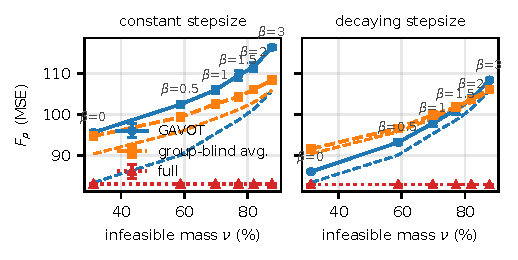
\includegraphics[width=\textwidth]{figs/severity_imdb.pdf}
\caption{IMDb-Wiki severity sweep: measured tail-500 (solid, $\pm1$ std)
against the exact floor $\Phi(\cdot)$ of each rule (dashed). Left, constant
stepsize: the residual swamps the alignment gain and transport loses
everywhere. Right, decaying: the curves track their floors and transport wins
until the floors close at high $\nu$.}
\vspace{-10pt}
\label{fig:severity}
\end{figure*}

\begin{figure*}[t]
\centering

\includegraphics[width=\textwidth]{figs/rare_group_fit.pdf}
\caption{Loss on the least represented group, decaying stepsize: Adult,
cross-entropy on race Other ($p_i=0.2$) against the observation exponent;
IMDb-Wiki, MSE on the $20$ top-importance identities, the least observed
once $\beta>0$. Same runs as Table~\ref{tab:overall}.}
\vspace{-10pt}
\label{fig:rare}
\end{figure*}

\noindent\textbf{E1: the headline cells.}
Table~\ref{tab:overall} reports the four headline instances. Transport wins
on three: Adult under prevalence availability,
$0.2269$ against $0.2479$ ($t{=}45$), and both IMDb cells, $86.06$ against
$91.63$ ($t{=}21$) and $84.28$ against $86.37$ ($t{=}13$); on Adult aligned
the two coincide at the oracle value, as Proposition~\ref{prop:surrogate}
predicts when $\tilde p=p$. Self-normalized upsampling
recovers most of the gain and transport the rest ($t{=}5.8$, $2.6$ against it); downsampling never beats
it, and LDS, which reweights by label rarity rather than group observation,
trails even group-blind averaging. On the least represented group the
margin over upsampling widens ($77.0$ against $80.0$, $73.6$ against $75.6$
on IMDb-Wiki).

\noindent\textbf{E2: the least represented group.}
Fig.~\ref{fig:rare} reads the same runs on the group the target exists for.
On Adult, transport lowers the loss on race Other at every skew: $0.073$
against $0.119$ on the prevalence instance (full $0.031$), $0.031$ against
$0.035$ aligned, matching full. On IMDb-Wiki the top-importance identities show the crossover of
Table~\ref{tab:severity} one step earlier: transport wins at $\nu\le0.70$
($77.0$ against $86.4$ at $\nu{=}0.31$, full $72.2$; $73.6$ against $79.9$
aligned) and loses at the three most infeasible skews. The single most
starved group (largest $p_i/r_i$) is Other itself on Adult and the top
identity on IMDb-Wiki, $253$ against $331$ at $\nu{=}0.31$ (full $219$).

% ----------------------------------------------------------- Table 2
\begin{table}[t]
\centering
\caption{IMDb-Wiki severity sweep, decaying stepsize: $\Delta_{\mathrm{floor}}$
the alignment gain of Theorem~\ref{thm:infeasible}, \emph{gain} the measured
advantage of transport, $t$ its Welch statistic. The residual averages $1.9$;
the sign flips where $\Delta_{\mathrm{floor}}$ crosses it.}
\label{tab:severity}
\setlength{\tabcolsep}{3.0pt}
\begin{tabular}{ccccc}
\toprule
$\beta$ & $\nu$ & $\Delta_{\mathrm{floor}}$ & gain & $t$ \\
\midrule
$0$   & $0.31$ & $6.99$ & $\best{+5.57}$ & $20.7$ \\
$0.5$ & $0.59$ & $5.71$ & $\best{+3.46}$ & $11.3$ \\
$1.0$ & $0.70$ & $3.67$ & $\best{+2.05}$ & $5.4$ \\
$1.5$ & $0.77$ & $2.56$ & $+0.58$ & $1.1$ \\
$2.0$ & $0.82$ & $1.62$ & $-0.03$ & $-0.1$ \\
$3.0$ & $0.88$ & $0.02$ & $-2.28$ & $-7.9$ \\
\bottomrule
\end{tabular}
\vspace{-8pt}
\end{table}

\noindent\textbf{E3: the crossover, and where the sign comes from.}
On Adult (Table~\ref{tab:severity}, Fig.~\ref{fig:severity}) the measured gain tracks $\Delta_{\mathrm{floor}}$ within $4\%$ at
three of five skews and exceeds it at the two most infeasible ($0.0210$
against $0.0110$, $0.0181$ against $0.0144$). On IMDb-Wiki the gain sits below
the floor by a residual close to constant in $\beta$, mean $1.9$, and the
sign flips exactly where $\Delta_{\mathrm{floor}}$ crosses that value,
between $\beta{=}1.5$ ($2.56$, gain $+0.58$) and $\beta{=}2.0$ ($1.62$,
$-0.03$): Theorem~\ref{thm:infeasible} at finite $T$. The $\ell_1$ criterion
cannot: $\|p-\hat p\|_1<\|p-\tilde p\|_1$ in all eleven instances, the three
where transport loses or ties included.

\noindent\textbf{E4: why the sign flips.}
At constant stepsize (Fig.~\ref{fig:severity}, left) transport loses on all
six IMDb skews, by up to $7.9$. A
starved group has $p_i>r_i$, so $\hat p$ truncates at the observation rate;
as $\nu$ grows $\hat p$ and $\tilde p$ starve the same groups and the floors
converge ($\Delta_{\mathrm{floor}}$ from $6.99$ to $0.02$, both $105.9$ at
$\nu{=}0.88$). Transport still concentrates weight on a starved
group whenever it appears, so its variance about the mean is larger
(Lemma~\ref{lem:variance} bounds only the second moment), and at constant
stepsize the iterates sit on a noise floor proportional to it. Under
$\eta_t=\eta/(1+t/1000)$ that floor decays, the curves fall onto their
dashed floors, and what remains is the residual, $2.3$ at $\nu{=}0.88$, the
one significant loss.

\noindent\textbf{E5: risk aversion, and where it does not help.}
On a $10\times10$ $(\alpha,\gamma)$ grid the overall objective is minimized
on the $\gamma=1$ edge of every instance: risk aversion costs the average. It earns its keep once, on the worst race of
Adult under prevalence availability: \avotcvar{} at $(0.2,0.7)$ reaches
$0.3624$ against $0.3679$ for \avot{} and $0.3994$ for group-blind averaging. On the least represented group the layer
never helps: the grid's best rare-group loss is at $\gamma{=}1$ on all four
headline instances. CVaR tilts among the groups present in the batch, and the rare
group is absent from most; on top of transport it multiplies weights already
$p_i/r_i$ large and amplifies variance, not alignment.

% =====================================================================
